
\documentclass[12pt]{article}
\usepackage[utf8]{inputenc}
\usepackage{graphicx}
\usepackage{amsmath}
\usepackage[margin=1in]{geometry}
\usepackage{indentfirst}
\usepackage{amsfonts}
\usepackage[portuguese]{babel}
\usepackage{float}
\usepackage[usenames,dvipsnames]{color}







\begin{document}

\begin{titlepage}

\newcommand{\HRule}{\rule{\linewidth}{0.5mm}} 
\center 
 

\textsc{\LARGE universidade de coimbra}\\[1.5cm] % Name of your university/college
\textsc{\Large departamento de engenharia informática}\\[4cm] % Major heading such as course name
\textsc{\large compiladores}\\[1cm] % Minor heading such as course title


\HRule \\[0.5cm]
{ \huge \bfseries Compilador para a linguagem iJava}\\[0.4cm] 
\HRule \\[8cm]
 
\begin{minipage}{0.4\textwidth}
\begin{flushleft} \large
\emph{Autor:}\\
Bruno \textsc{Caceiro}  \\caceiro@student.dei.uc.pt
\end{flushleft}
\end{minipage}
~
\begin{minipage}{0.4\textwidth}
\begin{flushright} \large
\emph{Autor:} \\
David \textsc{Cardoso}  \\davidfpc@student.dei.uc.pt
\end{flushright}
\end{minipage}\\[2cm]



{\large \today}\\[3cm]

\vfill

\end{titlepage}



\section{Introdução}
Este projecto consiste no desenvolvimento de um compilador para a linguagem \emph{iJava} (imperative Java), que consiste num pequeno subconjunto da linguagem Java (versão 5.0). Os programas da linguagem \emph{iJava} são constituídos por uma única classe (a principal), contendo necessariamente um método \emph{main}, e podendo conter outros métodos e atributos, todos eles estáticos e (possivelmente) públicos.

O projecto foi estruturado em 3 fases, primeiramente foi feita a Análise Lexical, implementada na linguagem \emph{C} e utilizando a ferramenta \emph{lex}. A segunda fase consistiu na análise sintática, com a  construção da árvore de sintaxe abstrata e análise semântica (tabelas de símbolos, deteção de erros semânticos). No final foi feita a geração de código.

\begin{figure}[H]
       \centering
       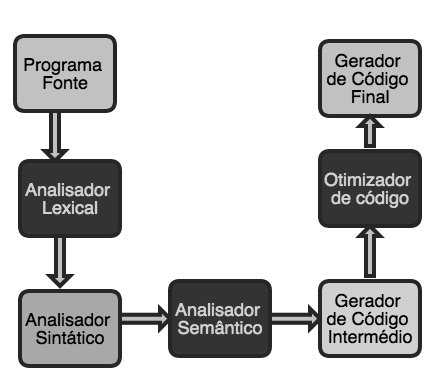
\includegraphics[keepaspectratio=true, width=300px]{fasesCompilacao.png}
       \caption{Fases de Compilação}
       \end{figure}


\section{Análise Lexical}

A Análise Lexical consiste em analisar a entrada de linhas de caracteres e produzir uma sequência de símbolos (\emph{tokens}) que podem ser manipulados mais facilmente por um \emph{parser}. É uma forma de verificar um determinado alfabeto, neste caso o alfabeto da linguagem \emph{iJava}.
Esta análise pode ser dividida em três fases:
\begin{itemize}
	\item Extração e classificação de \emph{tokens};
	\item Eliminação de delimitadores e comentários;
	\item Tratamento de erros;
\end{itemize}


\subsection{Tokens}
\begin{itemize}
	        \item \textbf{ID:} Sequências alfanuméricas começadas por uma letra, onde os símbolos "\_" e "\$" contam como letras. Maiúsculas e minúsculas são consideradas letras diferentes 
	        \item \textbf{INTLIT:} Sequências de dígitos decimais e sequências de dígitos hexadecimais (incluindo a-f e A-F) precedidas de "0x"
	        \item \textbf{BOOLLIT:} "true" \text{\textbar} "false" 
	        \item \textbf{INT:} "int"
	        \item \textbf{BOOL:} "boolean"
	        \item \textbf{NEW:} "new"
	        \item \textbf{IF:} "if"
	        \item \textbf{ELSE:} "else"
	        \item \textbf{WHILE:} "while"
	        \item \textbf{PRINT:} "System.out.println"
	        \item \textbf{PARSEINT:} "Integer.parseInt"
	        \item \textbf{CLASS:} "class"
	        \item \textbf{PUBLIC:} "public"
	        \item \textbf{STATIC:} "static"
	        \item \textbf{VOID:} "void"
	        \item \textbf{STRING:} "String"
	        \item \textbf{DOTLENGTH:} ".length"
	        \item \textbf{RETURN:} "return"
	        \item \textbf{OCURV:} "("
	        \item \textbf{CCURV:} ")"
	        \item \textbf{OBRACE} "\{"
	        \item \textbf{CBRACE:} "\}"
	        \item \textbf{OSQUARE:} "["
	        \item \textbf{CSQUARE:} "]"	 
	      \end{itemize}
	      \pagebreak
	    Foi necessário separar alguns \emph{tokens} devido às diferentes prioridades que cada operador tem.
		\begin{itemize}  
	        \item \textbf{OP1:} "\&\&"  
	        \item \textbf{OP1OR:} "\text{\textbar} \text{\textbar}"
	        \item \textbf{OP2:} "\textless" \text{\textbar} "\textgreater" \text{\textbar} "\textless=" \text{\textbar} "\textgreater="
	        \item \textbf{OP2EQS:} "==" \text{\textbar} "!="	        
	        \item \textbf{OP3:} "+" \text{\textbar} "-"
	        \item \textbf{OP4:} "*" \text{\textbar} "/" \text{\textbar} "\%"
	        \item \textbf{NOT:} "!"
	        \item \textbf{ASSIGN:} "="
	        \item \textbf{SEMIC:} ";"
	        \item \textbf{COMMA:} ","
	        \item \textbf{RESERVED:} O \emph{iJava} é um subconjunto da linguagem \emph{Java}, como tal, existe um conjunto de funcionalidades que embora não sejam suportadas, têm de ser consideradas. Assim, foi necessário tratar todo um conjunto de palavras reservadas de forma a permitir que sejam lexicalmente válidas mas não sintaticamente. 
	       	            \begin{itemize}
	       	                \item abstract
	       	                \text{\textbar} assert 
	       	                \text{\textbar} break 
	       	                \text{\textbar} byte 
	       	                \text{\textbar} case 
	       	                \text{\textbar} catch 
	       	                \text{\textbar} char 
	       	                \text{\textbar} const 
	       	                \text{\textbar} continue
	       	                 \text{\textbar} default 
	       	                 \text{\textbar} do 
	       	                 \text{\textbar} double
	       	                 \text{\textbar} enum 
	       	                 \text{\textbar} extends 
	       	                 \text{\textbar} final 
	       	                 \text{\textbar} finally 
	       	                 \text{\textbar} float 
	       	                 \text{\textbar} for 
	       	                 \text{\textbar} goto 
	       	                 \text{\textbar} implements 
	       	                 \text{\textbar} import 
	       	                 \text{\textbar} instanceof
	       	                 \text{\textbar} interface 
	       	                 \text{\textbar} long
	       	                 \text{\textbar} native
	       	                 \text{\textbar} package
	       	                 \text{\textbar} private 
	       	                 \text{\textbar} protected 
	       	                 \text{\textbar} short 
	       	                 \text{\textbar} strictfp
	       	                 \text{\textbar} super 
	       	                 \text{\textbar} switch 
	       	                 \text{\textbar} synchronized 
	       	                 \text{\textbar} this 
	       	                 \text{\textbar} throw 
	       	                 \text{\textbar} throws 
	       	                 \text{\textbar} transient 
	       	                 \text{\textbar} try
	       	                 \text{\textbar} volatile
		       	             \text{\textbar} null
	       	                 \text{\textbar} ++
	       	                 \text{\textbar} --
	       	            \end{itemize}      	        
		\end{itemize}
		
		
		\subsubsection{Tratamento de Erros}
		Se forem detectados erros lexicais no ficheiro de entrada então é impressa uma mensagem de erro no \emph{stdout}:
		\begin{itemize}
            \item "Line\textless num linha\textgreater,col\textless num coluna\textgreater:illegal character('\textless c \textgreater'\textbackslash n)"
            \item "Line\textless num linha\textgreater,col\textless num coluna\textgreater:unterminated comment\textbackslash n"
        \end{itemize}
		






\section{Análise Sintática e Semântica}

\subsection{Árvore de Sintaxe Abstrata}

\subsection{Tratamento de Erros Lexicais}

\subsection{Análise Semântica}

\subsection{Tabela de Símbolos}

\subsection{Tratamento de Erros Semânticos}









	
	


\end{document}